\documentclass{standalone}
\usepackage{tikz}
\usetikzlibrary{arrows}
\usetikzlibrary{positioning}
\usetikzlibrary{shapes.geometric}
\usepackage{amsmath}
\begin{document}
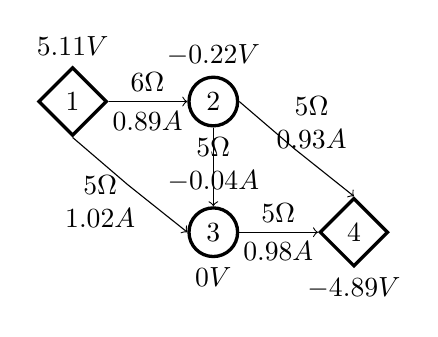
\begin{tikzpicture}[
endnode/.style={diamond, draw=black, fill=none, very thick, minimum size=1em},
node/.style={circle, draw=black, fill=none, very thick, minimum size=1em},
]
\node[endnode, label={$5.11V$}](n1){1};
\node[node, label={$-0.22V$}](n2)[right=of n1]{2};
\node[node, label=below:{$0V$}](n3)[below=of n2]{3};
\node[endnode, label=below:{$-4.89V$}](n4)[right=of n3]{4};
\draw[->] (n1.east) -- node[above]{$6\Omega$}++(0.99,0) -- node{}++(-0.99,0) -- node[below]{$0.89A$}++(0.99,0) -- (n2.west);
\draw[->] (n3.east) -- node[above]{$5\Omega$}++(0.99,0) -- node{}++(-0.99,0) -- node[below]{$0.98A$}++(0.99,0) -- (n4.west);
\draw[->] (n2.south) -- node[]{$\begin{matrix}5\Omega\\-0.04A\end{matrix}$}++(0,-0.99) -- (n3.north);
\draw[->] (n1.south) -- node[below]{$\begin{matrix}5\Omega\\1.02A\end{matrix}$}++(0.7,-0.6) -- (n3.west);
\draw[->] (n2.east) -- node[right]{$\begin{matrix}5\Omega\\0.93A\end{matrix}$}++(0.7,-0.6) -- (n4.north);
\end{tikzpicture}
\end{document}

